% Options for packages loaded elsewhere
\PassOptionsToPackage{unicode}{hyperref}
\PassOptionsToPackage{hyphens}{url}
%
\documentclass[
  11pt,
]{article}
\usepackage{amsmath,amssymb}
\usepackage{setspace}
\usepackage{iftex}
\ifPDFTeX
  \usepackage[T1]{fontenc}
  \usepackage[utf8]{inputenc}
  \usepackage{textcomp} % provide euro and other symbols
\else % if luatex or xetex
  \usepackage{unicode-math} % this also loads fontspec
  \defaultfontfeatures{Scale=MatchLowercase}
  \defaultfontfeatures[\rmfamily]{Ligatures=TeX,Scale=1}
\fi
\usepackage{lmodern}
\ifPDFTeX\else
  % xetex/luatex font selection
    \setmainfont[]{Arial}
\fi
% Use upquote if available, for straight quotes in verbatim environments
\IfFileExists{upquote.sty}{\usepackage{upquote}}{}
\IfFileExists{microtype.sty}{% use microtype if available
  \usepackage[]{microtype}
  \UseMicrotypeSet[protrusion]{basicmath} % disable protrusion for tt fonts
}{}
\makeatletter
\@ifundefined{KOMAClassName}{% if non-KOMA class
  \IfFileExists{parskip.sty}{%
    \usepackage{parskip}
  }{% else
    \setlength{\parindent}{0pt}
    \setlength{\parskip}{6pt plus 2pt minus 1pt}}
}{% if KOMA class
  \KOMAoptions{parskip=half}}
\makeatother
\usepackage{xcolor}
\usepackage[margin=2.5cm]{geometry}
\usepackage{longtable,booktabs,array}
\usepackage{calc} % for calculating minipage widths
% Correct order of tables after \paragraph or \subparagraph
\usepackage{etoolbox}
\makeatletter
\patchcmd\longtable{\par}{\if@noskipsec\mbox{}\fi\par}{}{}
\makeatother
% Allow footnotes in longtable head/foot
\IfFileExists{footnotehyper.sty}{\usepackage{footnotehyper}}{\usepackage{footnote}}
\makesavenoteenv{longtable}
\usepackage{graphicx}
\makeatletter
\newsavebox\pandoc@box
\newcommand*\pandocbounded[1]{% scales image to fit in text height/width
  \sbox\pandoc@box{#1}%
  \Gscale@div\@tempa{\textheight}{\dimexpr\ht\pandoc@box+\dp\pandoc@box\relax}%
  \Gscale@div\@tempb{\linewidth}{\wd\pandoc@box}%
  \ifdim\@tempb\p@<\@tempa\p@\let\@tempa\@tempb\fi% select the smaller of both
  \ifdim\@tempa\p@<\p@\scalebox{\@tempa}{\usebox\pandoc@box}%
  \else\usebox{\pandoc@box}%
  \fi%
}
% Set default figure placement to htbp
\def\fps@figure{htbp}
\makeatother
\setlength{\emergencystretch}{3em} % prevent overfull lines
\providecommand{\tightlist}{%
  \setlength{\itemsep}{0pt}\setlength{\parskip}{0pt}}
\setcounter{secnumdepth}{5}
% definitions for citeproc citations
\NewDocumentCommand\citeproctext{}{}
\NewDocumentCommand\citeproc{mm}{%
  \begingroup\def\citeproctext{#2}\cite{#1}\endgroup}
\makeatletter
 % allow citations to break across lines
 \let\@cite@ofmt\@firstofone
 % avoid brackets around text for \cite:
 \def\@biblabel#1{}
 \def\@cite#1#2{{#1\if@tempswa , #2\fi}}
\makeatother
\newlength{\cslhangindent}
\setlength{\cslhangindent}{1.5em}
\newlength{\csllabelwidth}
\setlength{\csllabelwidth}{3em}
\newenvironment{CSLReferences}[2] % #1 hanging-indent, #2 entry-spacing
 {\begin{list}{}{%
  \setlength{\itemindent}{0pt}
  \setlength{\leftmargin}{0pt}
  \setlength{\parsep}{0pt}
  % turn on hanging indent if param 1 is 1
  \ifodd #1
   \setlength{\leftmargin}{\cslhangindent}
   \setlength{\itemindent}{-1\cslhangindent}
  \fi
  % set entry spacing
  \setlength{\itemsep}{#2\baselineskip}}}
 {\end{list}}
\usepackage{calc}
\newcommand{\CSLBlock}[1]{\hfill\break\parbox[t]{\linewidth}{\strut\ignorespaces#1\strut}}
\newcommand{\CSLLeftMargin}[1]{\parbox[t]{\csllabelwidth}{\strut#1\strut}}
\newcommand{\CSLRightInline}[1]{\parbox[t]{\linewidth - \csllabelwidth}{\strut#1\strut}}
\newcommand{\CSLIndent}[1]{\hspace{\cslhangindent}#1}
\AtBeginDocument{\let\maketitle\relax}
\usepackage{graphicx}
\usepackage{setspace}
\usepackage{titlesec}
\usepackage{fancyhdr}
\usepackage{tocloft}
\usepackage{caption}
\captionsetup{font={normalsize,stretch=1.5}, labelfont=bf}
\captionsetup{font={small}, labelfont=bf}
\captionsetup[table]{position=bottom,skip=6pt}
\usepackage{subcaption}
\usepackage[titletoc,title]{appendix}
\usepackage{chngcntr}
\usepackage{amsmath}
\usepackage[hidelinks]{hyperref}
\usepackage{acro}
\usepackage{booktabs}
\usepackage{float}
\usepackage[section]{placeins}
\usepackage{threeparttable}
\usepackage[dvipsnames]{xcolor}
\usepackage{amssymb}
\usepackage{pifont}
\usepackage{etoolbox}
\AtBeginEnvironment{equation}{\setlength{\abovedisplayskip}{8pt}\setlength{\belowdisplayskip}{8pt}}
\AtBeginEnvironment{align}{\setlength{\abovedisplayskip}{8pt}\setlength{\belowdisplayskip}{8pt}}
\AtBeginEnvironment{subequations}{\setlength{\abovedisplayskip}{8pt}\setlength{\belowdisplayskip}{8pt}}
\newcommand{\robstrong}{\textcolor{ForestGreen}{\checkmark}}
\newcommand{\robmixed}{\textcolor{BurntOrange}{\(\triangle\)}}
\newcommand{\robweak}{\textcolor{BrickRed}{\ding{55}}}
\acsetup{first-style=long-short}
\acsetup{list/heading=section*, make-links=true}
\acsetup{make-links=true}
\pagestyle{plain}
\renewcommand{\cftsecfont}{\normalfont}
\renewcommand{\cftsecpagefont}{\normalfont}
\renewcommand{\cftsubsecindent}{1.5em}
\cftsetpnumwidth {2.5em}
\cftsetrmarg{3em}
\renewcommand{\cftsecleader}{\cftdotfill{\cftdotsep}}
\renewcommand{\cftsubsecleader}{\cftdotfill{\cftdotsep}}
\renewcommand{\cftloftitlefont}{\Large\bfseries\raggedright}
\renewcommand{\cftafterloftitle}{\par}
\DeclareAcronym{vix}{  short = VIX,  long = CBOE Volatility Index, tag = abbrev }
\DeclareAcronym{vxo}{  short = VXO,  long = CBOE S\&P100 Implied-Volatility Index, tag = abbrev }
\DeclareAcronym{jln}{  short = JLN,  long = Jurado–Ludvigson–Ng Macroeconomic Uncertainty Index, tag = abbrev }
\DeclareAcronym{tvar}{ short = TVAR, long = Threshold Vector Autoregression, tag = abbrev }
\DeclareAcronym{var}{  short = VAR,  long = Vector Autoregression, tag = abbrev }
\DeclareAcronym{svar}{ short = SVAR, long = Structural Vector Autoregression, tag = abbrev }
\DeclareAcronym{irf}{  short = IRF,  long = Impulse Response Function, tag = abbrev }
\DeclareAcronym{girf}{ short = GIRF, long = Generalized Impulse Response Function, tag = abbrev }
\DeclareAcronym{fevd}{ short = FEVD, long = Forecast-Error Variance Decomposition, tag = abbrev }
\DeclareAcronym{gfevd}{short = GFEVD,long = Generalized Forecast-Error Variance Decomposition, tag = abbrev }
\DeclareAcronym{bic}{  short = BIC,  long = Bayesian Information Criterion, tag = abbrev }
\DeclareAcronym{ols}{  short = OLS,  long = Ordinary Least Squares, tag = abbrev }
\DeclareAcronym{gfc}{  short = GFC,  long = Global Financial Crisis, tag = abbrev}
\DeclareAcronym{ltcm}{  short = LCTM,  long = Long-Term Capital Management, tag = abbrev}
\DeclareAcronym{sigma}{short = \ensuremath{\sigma},long  = volatility (std. dev.),tag = symbols}
\DeclareAcronym{tau}{short = \ensuremath{\tau},long  = threshold parameter,tag = symbols}
\DeclareAcronym{cstar}{short = \ensuremath{c^{*}},long  = BIC-optimal threshold,tag = symbols}
\DeclareAcronym{R_t}{short = \ensuremath{\mathcal{R}_t},long  = regime indicator at time $t$,tag = symbols}
\DeclareAcronym{Hmax}{short = \ensuremath{H_{\max}},long  = maximum IRF horizon,tag = symbols}
\DeclareAcronym{r_it}{short=\ensuremath{r_{i,t}}, long=percent log return of commodity $i$ at time $t$, tag=symbols}
\DeclareAcronym{P_it}{short=\ensuremath{P_{i,t}}, long=price level of commodity $i$ at time $t$, tag=symbols}
\DeclareAcronym{q_t}{short=\ensuremath{q_t}, long=raw uncertainty proxy (volatility or JLN) at time $t$, tag=symbols}
\DeclareAcronym{qbar}{short=\ensuremath{\bar q}, long=in-sample mean of the uncertainty proxy, tag=symbols}
\DeclareAcronym{s_q}{short=\ensuremath{s_q}, long=normalization scale,   tag=symbols}
\DeclareAcronym{qtilde_t}{short=\ensuremath{\tilde q_t}, long=standardized uncertainty proxy, tag=symbols}
\DeclareAcronym{qtilde_tm}{short=\ensuremath{\tilde q_t^{(m)}}, long=$m$-month moving average, tag=symbols}
\DeclareAcronym{m_win}{short=\ensuremath{m}, long=length of the smoothing window (months), tag=symbols}
\DeclareAcronym{d_delay}{short=\ensuremath{d}, long=threshold delay used in regime assignment, tag=symbols}
\DeclareAcronym{c_thr}{short=\ensuremath{c}, long=candidate threshold value, tag=symbols}
\DeclareAcronym{C_tau}{short=\ensuremath{C_{\tau}}, long=search interval for the threshold, tag=symbols}
\DeclareAcronym{Q_alpha}{short=\ensuremath{Q_{\alpha}(\cdot)}, long=quantile operator at probability $\alpha$, tag=symbols}
\DeclareAcronym{s_t}{short=\ensuremath{s_t}, long=binary regime state, tag=symbols}
\DeclareAcronym{dtc}{short=\ensuremath{d_t(c)}, long=indicator, tag=symbols}
\DeclareAcronym{Tset}{short=\ensuremath{\mathcal T}, long=time-index set of the sample, tag=symbols}
\DeclareAcronym{Trep}{short=\ensuremath{\mathcal T^{\mathrm{rep}}}, long=replication-window index set, tag=symbols}
\DeclareAcronym{Text}{short=\ensuremath{\mathcal T^{\mathrm{ext}}}, long=extended-window index set, tag=symbols}
\DeclareAcronym{Tlen}{short=\ensuremath{T}, long=number of observations in $\mathcal T$, tag=symbols}
\DeclareAcronym{Tone}{short=\ensuremath{T_{1}}, long=observations in the high-uncertainty regime, tag=symbols}
\DeclareAcronym{Hc}{short=\ensuremath{H(c)}, long=index set of high-regime times given threshold $c$, tag=symbols}
\DeclareAcronym{Lc}{short=\ensuremath{L(c)}, long=complement set $\mathcal T \setminus H(c)$, tag=symbols}
\DeclareAcronym{sH}{short=\ensuremath{s_H}, long=share of high-regime observations, tag=symbols}
\DeclareAcronym{dsH}{short=\ensuremath{\delta s_H}, long=difference in $s_H$ across uncertainty proxies, tag=symbols}
\DeclareAcronym{y_vec}{short=\ensuremath{\mathbf y_t}, long=vector of endogenous variables at time $t$, tag=symbols}
\DeclareAcronym{alpha_st}{short=\ensuremath{\boldsymbol{\alpha}(s_t)}, long=regime-dependent intercept vector, tag=symbols}
\DeclareAcronym{Aks}{short=\ensuremath{A_k(s_t)}, long=regime-dependent VAR coefficient matrix at lag $k$, tag=symbols}
\DeclareAcronym{p_ord}{short=\ensuremath{p}, long=VAR lag order, tag=symbols}
\DeclareAcronym{eps_t}{short=\ensuremath{\boldsymbol{\varepsilon}_t}, long=innovation (reduced-form shock) at time $t$, tag=symbols}
\DeclareAcronym{Sigma_st}{short=\ensuremath{\Sigma(s_t)}, long=regime-dependent covariance matrix of $\boldsymbol{\varepsilon}_t$, tag=symbols}
\DeclareAcronym{Zs}{short=\ensuremath{Z_s}, long=regime-$s$ regressor matrix in OLS, tag=symbols}
\DeclareAcronym{Ys}{short=\ensuremath{Y_s}, long=regime-$s$ stacked dependent variable matrix, tag=symbols}
\DeclareAcronym{Bs}{short=\ensuremath{B^{(s)}(c)}, long=OLS coefficient matrix estimated in regime $s$ at threshold $c$, tag=symbols}
\DeclareAcronym{Ts}{short=\ensuremath{T_s}, long=number of observations in regime $s$, tag=symbols}
\DeclareAcronym{kcpd}{short=\ensuremath{k(c,p,d)}, long=parameter count, tag=symbols}
\DeclareAcronym{eta_is}{short=\ensuremath{\eta_i^{(s)}}, long=shock to variable $i$ normalized by its s.d. in regime $s$, tag=symbols}
\DeclareAcronym{sig_is}{short=\ensuremath{\sigma_i^{(s)}}, long=standard deviation of innovation $i$ in regime $s$, tag=symbols}
\DeclareAcronym{e_i}{short=\ensuremath{e_i}, long=$i$-th unit vector, tag=symbols}
\DeclareAcronym{i_idx}{short=\ensuremath{i}, long=index of the shocked variable, tag=symbols}
\DeclareAcronym{ell_idx}{short=\ensuremath{\ell}, long=index of the responding variable, tag=symbols}
\DeclareAcronym{h_hor}{short=\ensuremath{h}, long=impulse-response horizon (periods), tag=symbols}
\DeclareAcronym{Hcap}{short=\ensuremath{H}, long=horizon cutoff used for cumulative measures, tag=symbols}
\DeclareAcronym{Hmax2}{short=\ensuremath{H_{\max}}, long=maximum horizon, tag=symbols}
\DeclareAcronym{n_dim}{short=\ensuremath{n}, long=VAR dimension (number of variables), tag=symbols}
\DeclareAcronym{B_boot}{short=\ensuremath{B}, long=number of Monte Carlo/boostrap draws, tag=symbols}
\DeclareAcronym{info_tm1}{short=\ensuremath{\mathcal I_{t-1}}, long=information set, tag=symbols}
\DeclareAcronym{s_set}{short=\ensuremath{s\in\{0,1\}}, long=regime label, tag=symbols}
\DeclareAcronym{GIRFsym}{short=\ensuremath{\mathrm{GIRF}^{\,i\to \ell,(s)}(h)}, long=generalized impulse response, tag=symbols}
\DeclareAcronym{GIRFhat}{short=\ensuremath{\widehat{\mathrm{GIRF}}_{i\to \ell}^{(s)}(h)}, long=Monte Carlo estimate of the GIRF, tag=symbols}
\DeclareAcronym{DeltaIRF}{short=\ensuremath{\Delta\mathrm{IRF}^{\,i\to \ell}(h)}, long=difference in GIRFs between high and low regimes, tag=symbols}
\DeclareAcronym{hhalf}{short=\ensuremath{h_{1/2}^{(s)}(i\to \ell)}, long=half-life (time to half the peak response) in regime $s$, tag=symbols}
\DeclareAcronym{Deltahhalf}{short=\ensuremath{\Delta h_{1/2}(g)}, long=group-level difference in half-life between proxies, tag=symbols}
\DeclareAcronym{GFEVDhat}{short=\ensuremath{\widehat{\mathrm{GFEVD}}_{\ell,i}^{(s)}(H)}, long=generalized FEVD share of shock, tag=symbols}
\DeclareAcronym{GFEVDg}{short=\ensuremath{\mathrm{GFEVD}_g^{(\cdot,\cdot)}(H)}, long=group-aggregated GFEVD, tag=symbols}
\DeclareAcronym{Ramp}{short=\ensuremath{R_{\mathrm{amp}}^{\,i\to \ell}}, long=amplitude ratio (low vs high regime peak), tag=symbols}
\DeclareAcronym{AreaDiff}{short=\ensuremath{A^{\,i\to \ell}(H)}, long=area difference of responses (high minus low), tag=symbols}
\DeclareAcronym{Jacc}{short=\ensuremath{J}, long=overlap index (Jaccard) of volatility and JLN high regimes, tag=symbols}
\DeclareAcronym{DDg}{short=\ensuremath{\Delta\Delta_g(H)}, long=double difference of group GFEVDs across proxies and regimes, tag=symbols}
\DeclareAcronym{UgP}{short=\ensuremath{U_g^{(p)}}, long=percentile-based group contrast (volatility minus JLN), tag=symbols}
\DeclareMathOperator*{\argmin}{arg\,min}
\DeclareMathOperator{\diag}{diag}
\newcommand{\E}{\mathbb{E}}
\usepackage{booktabs}
\usepackage{longtable}
\usepackage{array}
\usepackage{multirow}
\usepackage{wrapfig}
\usepackage{float}
\usepackage{colortbl}
\usepackage{pdflscape}
\usepackage{tabu}
\usepackage{threeparttable}
\usepackage{threeparttablex}
\usepackage[normalem]{ulem}
\usepackage{makecell}
\usepackage{xcolor}
\usepackage{bookmark}
\IfFileExists{xurl.sty}{\usepackage{xurl}}{} % add URL line breaks if available
\urlstyle{same}
\hypersetup{
  hidelinks,
  pdfcreator={LaTeX via pandoc}}

\author{}
\date{\vspace{-2.5em}}

\begin{document}

\setstretch{1.5}
\begin{titlepage}
\thispagestyle{empty}
\begin{center}
\vspace*{2cm}
{\LARGE \textbf{The Nonlinear Effects of Macroeconomic Uncertainty on\\
Commodity Price Returns: A Replication and Extension of Joets \& Mignon (2016)}}\\[2cm]

{\large Simon Ochmann}\\[1.5cm]

30 August 2025
\end{center}
\end{titlepage}

\pagenumbering{Roman}
\setcounter{page}{2}

\begin{center}\bfseries Abstract\end{center}

\noindent
This paper investigates how the transmission of shocks to commodity-market return depends on the level and type of macroeconomic uncertainty by replicating and extending Joets \& Mignon (\citeproc{ref-joetsDoesVolatilityCommodity2016}{2016}). The replication estimates a two-regime \ac{tvar} over 1986--2015 using the \ac{vxo}. To extend the sample through June 2025, the \ac{vix} is employed from 1990 onward, for 1986--1989, when VIX is unavailable, VXO is used. To capture broader, predictability-based uncertainty, the \ac{jln} macroeconomic uncertainty index is incorporated across the full 1986--2025 period. Robustness is benchmarked against linear VAR and structural VAR specifications while varying lag length, threshold selection, and bootstrap confidence intervals. Sensitivity analyses contrast volatility-based (VXO/VIX) with predictability-based (JLN) proxies to assess proxy dependence. This design isolates state-dependent transmission of shocks to the commodity system conditional on the uncertainty.

\clearpage

\phantomsection
\addcontentsline{toc}{section}{Contents}
\tableofcontents
\clearpage

\phantomsection
\addcontentsline{toc}{section}{List of Figures}
\listoffigures
\clearpage

\phantomsection
\addcontentsline{toc}{section}{List of Tables}
\listoftables
\clearpage

\phantomsection
\addcontentsline{toc}{section}{List of Symbols}
\small
\printacronyms[
  name=List of Symbols,
  include=symbols,
  heading=section*,
  display=all,
  pages={display=first, fill=\dotfill, name=false, seq/use=false}
]
\clearpage

\phantomsection
\addcontentsline{toc}{section}{List of Abbreviations}
\small
\printacronyms[
  name=List of Abbreviations,
  include=abbrev,
  heading=section*,
  display=used,
  pages={display=first, name=false, seq/use=false}
]
\acresetall
\clearpage

\pagenumbering{arabic}
\setcounter{page}{1}

\section{Introduction}\label{introduction}

Macroeconomic uncertainty can reshape how shocks propagate to commodity markets, with consequences for risk management, asset allocation, and policy design. Because commodity returns load on real-side disturbances and on financial conditions, the mapping from uncertainty to volatility is unlikely to be linear. When uncertainty is elevated, transmission may switch regimes, amplifying variance and tail risk in ways a pooled linear model cannot capture. Building on the nonlinear evidence in Joets \& Mignon (\citeproc{ref-joetsDoesVolatilityCommodity2016}{2016}), this paper studies such state-dependent transmission in a two-regime Threshold VAR for 18 monthly commodities spanning energy, precious metals, industrial metals, and agriculture. The replication window covers 1986--2015, as in the original study, and the analysis is extended through June 2025.

The analysis is organized around three research questions: (i) does the original state-contingent amplification result replicate on the 1986--2015 window, (ii) how do findings change when the sample is extended through June 2025, and (iii) to what extent does proxy choice volatility-based VXO/VIX versus macro based Jurado Ludvigson Ng (JLN) uncertainty alter regime identification and the measured size and persistence of volatility spillovers?
To ensure continuous coverage, the study implements a proxy handover from the CBOE S\&P100 Volatility Index VXO (1986--1989) to the CBOE S\&P500 Volatility Index (VIX) from 1990 onward. In parallel, the JLN macroeconomic uncertainty index is incorporated over the full 1986--2025 sample to represent a conceptually distinct, predictability based measure of uncertainty.

Methodologically, the paper estimates two-regime TVARs in which the smoothed, lagged proxy governs the regime indicator. Lag order and delay are selected using by pooled information criteria and stability constraints to avoid overfitting and spurious thresholds. Regime-specific dynamics are quantified via \ac{girf}, which allow for history dependent paths, and \ac{fevd}, which attribute volatility to commodity-system shocks conditional on uncertainty state. For discipline, a pooled linear VAR and a recursive \ac{svar} benchmark provide counterfactuals in which responses are constrained to be state-invariant Kilian \& Lütkepohl (\citeproc{ref-kilianStructuralVectorAutoregressive2017}{2017}). This setup delivers a transparent contrast between linear and nonlinear propagation without over-interpreting formal linearity tests in small samples.

The empirical design is motivated by two considerations that matter for both academic inference and decision use. First, different uncertainty proxies encode different information sets and investor beliefs. Option-implied volatility (VXO/VIX) is a forward-looking, market-priced gauge that can spike rapidly and embed risk-neutral probabilities, whereas the JLN index extracts macroeconomic predictability from large datasets under the physical measure and evolves more smoothly. If regime classification depends on the proxy, estimated responses and half-lives may diverge, especially around events such as the COVID-19 shock and the 2022--24 tightening cycle. Second, commodity markets are heterogeneous: energy and industrial metals tend to exhibit larger and more persistent responses than precious metals or agriculture. A multi-sector panel helps separate common uncertainty effects from sector-specific dynamics.

The contributions are twofold. First, the paper recovers the core nonlinear result of Joets \& Mignon (\citeproc{ref-joetsDoesVolatilityCommodity2016}{2016}), high-uncertainty regimes exhibit larger and longer-lived responses, while documenting stability and residual diagnostics (Table 1). Second, the paper extends the analysis through June 2025 and performs a proxy-comparison that demonstrates how volatility based (VXO/VIX) versus predictability-based (JLN) measures materially affect regime timing and the magnitude and persistence of volatility responses. This proxy dependence is not a technical footnote: it has first order implications for stress testing and risk management, where relying on a single proxy can under- or over-state commodity-market risk.

All results are generated from a packaged release with a frozen R environment (4.4.3), scripted data ingestion and transformations, deterministic random-seed control for simulation and bootstrap routines, and automated exports of figures and CSV artifacts. The full pipeline data, estimation, diagnostics, and output, runs end-to-end from a single orchestration script, enabling replication and facilitating extensions.

The remainder of the paper proceeds as follows. Section \ref{sec:data} describes the data, transformations, and uncertainty proxies. Section \ref{sec:econometric} details the econometric framework, threshold selection, and inference procedures. Section \ref{sec:replication} reports replication results for 1986--2015. Section \ref{sec:extension} presents the 1986--2025 extension and the proxy comparison. Section \ref{sec:validation} provides validation and robustness analyses. Section \ref{sec:discussion} discusses implications for stress testing, risk management, and policy calibration. Section \ref{sec:conclusion} concludes.

\subsection{Literature Review}\label{literature-review}

TVARs capture state-dependent dynamics via observed regime splitters Tong (\citeproc{ref-tongNonlinearTimeSeries1990}{1990}). Nonlinear impulse responses are computed with the Koop--Pesaran--Potter generalized method, averaging over future innovation paths (\citeproc{ref-koopImpulseResponseAnalysis1996}{Koop et al., 1996}), while order-invariant normalizations follow Pesaran \& Shin (\citeproc{ref-pesaranGeneralizedImpulseResponse1998}{1998}). For linear benchmarks and identification, standard VAR/SVAR expositions and practice are followed (\citeproc{ref-kilianStructuralVectorAutoregressive2017}{Kilian \& Lütkepohl, 2017}; \citeproc{ref-lutkepohlNewIntroducitonMultiple2005}{Lütkepohl, 2005}; \citeproc{ref-stockVectorAutoregressions2001}{Stock \& Watson, 2001}). As uncertainty measures, option-implied volatility (VXO/VIX) with macro-predictability JLN are used, reflecting distinct information sets. On commodities, the replication target is Joets \& Mignon (\citeproc{ref-joetsDoesVolatilityCommodity2016}{2016}), who emphasize nonlinear propagation to commodity markets in high-uncertainty states.

\section{Data \& Measurement}\label{sec:data}

This section documents the panel construction, uncertainty proxies, and preprocessing choices. The analysis relies on two families of inputs exported by the codebase in the frozen release consumed by this paper: (i) a monthly commodity-price panel transformed into returns, and (ii) the uncertainty proxies used as threshold variables. All paths resolve inside the selected release directory: figures are stored in /figures/decomposition/ or /artifacts/figures/decomposition/, and tidy CSV artifacts in /artifacts/data/. The analysis contrasts a volatility-based splitter (VXO/VIX) with a macro-predictability splitter (JLN).

\subsection{Commodity panel}\label{sec:dataone}

The dependent block comprises 18 benchmark commodities spanning energy, precious metals, industrial metals, and agriculture. Table A.1 lists the series and coverage. For each \(i = 1,\ldots,18\), a continuous monthly series is constructed from the World Bank Pink Sheet Commodity Markets, aligned to month-end and merged on the intersection of timestamps to ensure a balanced panel over the estimation window. Following Joets \& Mignon (\citeproc{ref-joetsDoesVolatilityCommodity2016}{2016}), the replication window begins in January 1986 to ensure availability of an implied volatility threshold, the extension carries the panel to June 2025.

For commodity \(i\) at month \(t\), returns are constructed as in Appendix \ref{app-formulas}, Eq. \eqref{eq:r-log-returns}.
Where indicated, series are standardized to \(z\)-scores within the relevant estimation window to equalize scale across commodities. No winsorization is applied: large moves around the \ac{gfc}, COVID-19, and the 2022--24 tightening are retained to preserve stressed-state information. Two file shapes are maintained, a long panel \{date, series ID, group, value\} for tidy summaries and decompositions, and a wide matrix with commodities as columns for VAR/TVAR estimation. Appendix A provides an inventory table documenting coverage by group.

\subsection{Uncertainty proxies and threshold design}\label{sec:datatwo}

Regimes are defined by an observed threshold variable \(q_t\). The design uses two conceptually distinct measures: (i) use a proxy available over the replication window (1986--2015) to make replication meaningful, (ii) use a conceptually distinct proxy to test measurement robustness on the 1986--2025 extension.
The replication uses the CBOE S\&P100 implied volatility index VXO (1986--2015). For the extension, a handover to the CBOE S\&P500 implied-volatility index VIX is implemented from January 1990 onward, 1986--1989 continues to use VXO. Because the underlyings differ (S\&P100 vs S\&P500), the splice is treated as a measurement switch, not a literal continuation. The Jurado--Ludvigson--Ng (JLN) index summarizes the expected forecast variance of a large macroeconomic panel at monthly frequency, offering a predictability-based view of uncertainty that can evolve more smoothly than option-implied risk.
Let \(q_t\) denote either VXO/VIX or JLN. The regime driver fed into the TVAR is constructed as:

\begin{subequations}\label{eq:tilde-q}
\begin{align}
\tilde{q}_t &= \frac{q_t - \bar{q}}{s_q}, \label{eq:tilde-q-level}\\
\tilde{q}_t^{(m)} &= \frac{1}{m}\sum_{j=0}^{m-1}\tilde{q}_{t-j}, \label{eq:tilde-q-smooth}\\
\mathcal{R}_t &= \mathbf{1}\!\left\{ \tilde{q}_t^{(m)} \ge \tau \right\}. \label{eq:tilde-q-regime}
\end{align}
\end{subequations}

Standardization is carried out within the relevant estimation window 1986--2015 for the replication and 1986--2025 for the extension. The baseline employs a 3 month smoother (\(m=3\)) and a one month delay (\(d=1\)) to temper event-month spikes and reduce simultaneity with commodity returns. For fixed \(p\) and \(d\), the selected threshold \(c^*\) minimizes \ac{bic}.

\begin{equation}\label{eq:c-star-argmin}
c^{*} = \arg\min_{c \in C_{\tau}} \mathrm{BIC}(c).
\end{equation}

Using both a volatility-based and a macro-based splitter makes proxy risk explicit: if VXO/VIX and JLN identify different high-uncertainty months, measured amplification is proxy-dependent. Regime incidence is therefore reported via regime-share diagnostics, and the high-state share \(s_H\) is defined in Appendix \ref{app-formulas}, Eq. \eqref{eq:s-h-big}.
A non-zero \(\delta_{s_H}\) signals economically meaningful differences in regime timing and foreshadows differences in the size and half-life of volatility spillovers critical for stress testing and drawdown protection.

\subsection{Samples, alignment, and diagnostics}\label{sec:datathree}

Because VXO (S\&P100) and VIX (S\&P500) are distinct option markets, the 1990 handover is treated as a measurement switch rather than a literal continuation. Two safeguards govern the splice: (i) standardization within each estimation window so thresholding depends on relative \(z\)-levels; and (ii) smoothing and lagging to mute event-month spikes and align information sets. The regime driver entering the TVAR is given by Appendix \ref{app-formulas}, Eq. \eqref{eq:tilde-q-t-2}. Replication and extension windows follow Appendix \ref{app-formulas}, Eq. \eqref{eq:mathcal-t}), the volatility specification uses VXO for 1986--1989 and VIX from 1990 onward, while JLN spans 1986--2025. All inputs are monthly and aligned to month-end.

Daily uncertainty measures are not mixed into the monthly TVAR to avoid timing conventions and aggregation artifacts. For any candidate threshold \(c\), the regime sets are \(H(c)\) and \(L(c)\) in Appendix \ref{app-formulas}, Eq. \eqref{eq:H-L-sets}. The grid search is trimmed so each regime contains at least 15\% of observations (see Appendix \ref{app-formulas}, Eq. \eqref{eq:c-in}). Post thresholding, each commodity must satisfy minimum coverage in both regimes (see Appendix \ref{app-formulas}, Eq. \eqref{eq:s-h}), the proxy differences \(\delta_{s_H}\) flags proxy-dependent timing.

Standardization within \(\mathcal{T}^{rep}\) and \(\mathcal{T}^{ext}\) ensures that any level shift at January 1990 does not mechanically change regime assignment. Diagnostics inspect (i) the distribution of \(\tilde{q_t}\) around the handover, (ii) local stability of \(s_H\) when perturbing \(c^*\) on a fine grid, and (iii) commodity-by-regime coverage. These checks, together with the regime-share figures and decomposition tables ingested from the release, make the sampling, alignment, and thresholding transparent and auditable.

\section{Econometric Framework}\label{sec:econometric}

The empirical strategy mirrors Joets \& Mignon (\citeproc{ref-joetsDoesVolatilityCommodity2016}{2016}): a replication on 1986--2015, an extension to 1986--2025, and validation against linear benchmarks and robustness grids. Nonlinearity is captured with a two-regime threshold VAR (TVAR) in which regime switches are governed by an observed uncertainty proxy. Shocks are analyzed with generalized impulse responses (GIRFs) suited to nonlinear dynamics, and contribution analysis proceeds via a state-contingent analogue of the forecast-error variance decomposition (FEVD).

\subsection{TVAR specification and regime definition}\label{sec:econometricone}

Let \(y_t \in \mathbb{R}^n\) stack monthly standardized returns for \(n=18\) commodities constructed in Section \ref{sec:data}. Define \(x_t\) as in Appendix \ref{app-formulas}, Eq. \eqref{eq:x-t} and the binary state \(s_t(c)\) as in Appendix \ref{app-formulas}, Eq. \eqref{eq:s-t-c}. Conditional on \(s_t\), a TVAR\((p)\) evolves as in Eq. \eqref{eq:y-t} Tong (\citeproc{ref-tongNonlinearTimeSeries1990}{1990}).

\begin{equation}\label{eq:y-t}
\begin{aligned}
\mathbf{y}_t &= \boldsymbol{\alpha}(s_t)
+ \sum_{k=1}^{p} A_k(s_t)\,\mathbf{y}_{t-k}
+ \boldsymbol{\varepsilon}_t, \\
\boldsymbol{\varepsilon}_t &\sim \mathcal{N}\!\bigl(\mathbf{0},\, \Sigma(s_t)\bigr).
\end{aligned}
\end{equation}

Estimation proceeds by regime-wise \ac{ols} after splitting the sample according to \(s_t(c)\). Let \(Z_t = [1,y_{t-1}^{\top},..., y_{t-p}^{\top}]^{\top}\). Stacking observations withing regime \(s\) yields the estimators in Appendix \ref{app-formulas}, Eq. \eqref{eq:b-s-c}, where \(T_s\) is the number of observations in regime \(s\). The search over \(c\) as restricted to the trimmed interval described in Section \ref{sec:datatwo} ensures adequate balance across regimes.

The triple \((c^*,p^*, d^* )\) minimizes a pooled \ac{bic} based on Gaussian likelihoods (see Appendix \ref{app-formulas}, Eq. \eqref{eq:bic}), see also (\citeproc{ref-lutkepohlNewIntroducitonMultiple2005}{Lütkepohl, 2005}). Stability requires the spectral radius of each regime's companion matrix to lie inside the unit circle, \(ρ(A^{(s)})<1\). As a descriptive contrast, a pooled VAR vs.~TVAR comparison indicates materially different coefficients, we therefore proceed with the state-dependent specification (\citeproc{ref-tsayTestingModelingMultivariate1998}{Tsay, 1998}).

\subsection{Shocks, GIRFs, and state-contingent FEVD}\label{sec:econometrictwo}

In nonlinear systems, the effect of a shock depends on the state in which it hits. Accordingly, impulse responses are computed using the Koop--Pesaran--Potter GIRF (\citeproc{ref-koopImpulseResponseAnalysis1996}{Koop et al., 1996}), which conditions on the pre-shock regime and averages over future innovation paths.To ensure order-invariant normalization and comparability within regime \(s\), a one-sigma generalized shock to variable \(i\) is

\begin{equation}\label{eq:n-i}
\begin{aligned}
\sigma_i^{(s)} &\equiv \sqrt{\Sigma_{ii}^{(s)}}, \\
\eta_i^{(s)}   &\equiv \frac{\Sigma^{(s)} e_i}{\sigma_i^{(s)}},
\end{aligned}
\end{equation}

where \(e_i\) is the \(i\)-th canonical unit vector and \(\Sigma^{(s)}\) is the regime-specific innovation covariance (\citeproc{ref-pesaranGeneralizedImpulseResponse1998}{Pesaran \& Shin, 1998}).For responsible variable \(\ell\) and horizon \(h\), the GIRF at pre-shock state \(s\) is

\begin{equation}\label{eq:girf}
\mathrm{GIRF}^{\,i \to \ell,(s)}(h)
=
\mathbb{E}\!\left[\, y_{\ell,t+h} \;\middle|\; \varepsilon_t=\eta_i^{(s)},\, s_t=s,\, \mathcal{I}_{t-1} \right]
-
\mathbb{E}\!\left[\, y_{\ell,t+h} \;\middle|\; \varepsilon_t=0,\, s_t=s,\, \mathcal{I}_{t-1} \right].
\end{equation}

with \(\mathcal{I}_{t-1}\) the observed pre-shock history. The Monte-Carlo estimator draws vector residuals within regime \(s\) the and averages over \(B\) replications(see Appendix \ref{app-formulas}, Eq. \eqref{eq:hatgirf}). Amplification is summarized by regime differences curves \(\Delta IRF\) (Eq. \eqref{eq:delta-irf}).

\begin{equation}\label{eq:delta-irf}
\Delta \mathrm{IRF}^{\,i \to \ell}(h)
=
\mathrm{GIRF}^{\,i \to \ell,(H)}(h)
-
\mathrm{GIRF}^{\,i \to \ell,(L)}(h).
\end{equation}

and regime-specific half-lives,

\begin{equation}\label{eq:h-1-2}
h_{1/2}^{(s)}(i \to \ell)
=
\min\left\{\, h \ge 0 \;:\;
\left|\mathrm{GIRF}^{\,i \to \ell,(s)}(h)\right|
\le
\frac{1}{2}\,
\max_{0 \le j \le H_{\max}}
\left|\mathrm{GIRF}^{\,i \to \ell,(s)}(j)\right|
\right\}.
\end{equation}

Because a nonlinear model has no single moving-average representation, the FEVD must also be computed state-contingently. Using the GIRFs, the generalized FEVD share contributed by shock \(i\) to variable \(\ell\) over Horizon \(H\) in regime \(s\) is

\begin{equation}\label{eq:gfevd}
\widehat{\mathrm{GFEVD}}_{\ell,i}^{(s)}(H)
=
\frac{\sum_{h=0}^{H} \bigl(\widehat{\mathrm{GIRF}}_{i \to \ell}^{(s)}(h)\bigr)^2}
     {\sum_{j=1}^{n}\sum_{h=0}^{H} \bigl(\widehat{\mathrm{GIRF}}_{j \to \ell}^{(s)}(h)\bigr)^2}.
\end{equation}

Group-level contributions for energy, precious, industrial, agriculture are obtained by summing the numerator across shocks \(i\) within each group and then normalizing. This construction mirrors generalized variance decompositions in linear VARs (\citeproc{ref-pesaranGeneralizedImpulseResponse1998}{Pesaran \& Shin, 1998}), but the conditioning on regime \(s\) makes it informative about stress-state transmission, precisely the object of interest for risk management. For readability, Section \ref{sec:replicationtwo} visualizes responses using regime‑split linear VARs. These plots are for qualitative orientation, direction and persistence only. All quantitative objects---TVAR GIRFs, ΔIRFs, and state‑contingent GFEVDs are computed from the TVAR per (\citeproc{ref-koopImpulseResponseAnalysis1996}{Koop et al., 1996}; \citeproc{ref-pesaranGeneralizedImpulseResponse1998}{Pesaran \& Shin, 1998}).

\subsection{Estimation, inference, benchmarks, and robustness}\label{sec:econometricthree}

Inference uses a regime-aware residual bootstrap (\citeproc{ref-kilianStructuralVectorAutoregressive2017}{Kilian \& Lütkepohl, 2017}). Fix \((c^*, p^*, d^*)\) resample vector residuals within each regime, simulate paths under the estimated TVAR, recompute GIRFs, \(\Delta{IRFs}\), and GFEVDs, and form percentile confidence bands. Seeds are fixed in the release for deterministic replication.
Two linear benchmarks anchor the nonlinear results. A pooled VAR \((p^*)\) on \(y_t\) delivers order-invariant generalized IRFs and closed-form GFEVDs (\citeproc{ref-lutkepohlNewIntroducitonMultiple2005}{Lütkepohl, 2005}). A recursive SVAR augments the VAR with the uncertainty proxy ordered last to identify a structural uncertainty shock under linear dynamics (\citeproc{ref-kilianStructuralVectorAutoregressive2017}{Kilian \& Lütkepohl, 2017}). The comparison is intentional: the TVAR quantifies state-contingent responses to generic shocks in the commodity system, whereas the SVAR isolates a linear uncertainty shock. Agreement in signs but larger magnitudes and longer half-lives in the TVAR's high-uncertainty regime indicate precisely what linear models miss.
Robustness is evaluated along four axes. (i) Lag/delay: \((p,d)\in\{2,\ldots,6\}\), with selections reported by proxy and sample window.(ii) Threshold perturbations: local moves around \(c^*\) within the trimmed set, documenting stability of sign, relative size, and half-life.(iii) Horizon:\(H\in\{12,24,36\}\) ensuring narratives do not hinge on a single horizon. (iv) Coverage and diagnostics: minimum observations by regime and commodity (Section \ref{sec:datathree}), regime-wise residual whiteness/heteroskedasticity checks, and companion-matrix stability. A compact table aggregates outcomes with \(✓/△/✗\) flags for sign, relative magnitude, and half-life stability, figures in Section 5 visualize regime-specific GIRFs, GFEVD stacks, and \(\Delta{IRFs}\).

\subsubsection{Model selection \& diagnostics}\label{sec:econometricthreeone}

Table 1 reports the selected \((p, d, c^*)\), regime balance, stability \((\lambda max)\), residual whiteness (LB\(p\)), and a descriptive sup-LM contrast versus a pooled VAR (\citeproc{ref-kilianStructuralVectorAutoregressive2017}{Kilian \& Lütkepohl, 2017}; \citeproc{ref-lutkepohlNewIntroducitonMultiple2005}{Lütkepohl, 2005})

\begin{table}[!h]
\centering
\caption[Model selection \& diagnostics]{\label{tab:tbl1render}\label{tab:tblX} Model selection and diagnostics by window and proxy: selected lag $p$, delay $d$, threshold $c^*$, regime counts/shares, stability (spectral radius), Ljung–Box residual whiteness (min $p$ across variables), and descriptive sup-LM linearity contrast.}
\centering
\resizebox{\ifdim\width>\linewidth\linewidth\else\width\fi}{!}{
\fontsize{9}{11}\selectfont
\begin{threeparttable}
\begin{tabular}[t]{llrrrrrlllllll}
\toprule
Window & Proxy & p & d & c* & T (low) & T (high) & s(H) & lambda max (L) & lambda max (H) & LB p (L) & LB p (H) & sup-LM stat & sup-LM p\\
\midrule
\cellcolor{gray!10}{Extension (1986–2025)} & \cellcolor{gray!10}{JLN (macro uncertainty)} & \cellcolor{gray!10}{2} & \cellcolor{gray!10}{1} & \cellcolor{gray!10}{0.961} & \cellcolor{gray!10}{357} & \cellcolor{gray!10}{63} & \cellcolor{gray!10}{15.0\%} & \cellcolor{gray!10}{0.581} & \cellcolor{gray!10}{0.881} & \cellcolor{gray!10}{0.002} & \cellcolor{gray!10}{0.001} & \cellcolor{gray!10}{5,055} & \cellcolor{gray!10}{<1e-12}\\
Extension (1986–2025) & Volatility (VXO->VIX) & 2 & 2 & 26.834 & 318 & 59 & 15.6\% & 0.578 & 0.970 & 0.014 & 0.009 & 5,251 & <1e-12\\
\cellcolor{gray!10}{1990-01 to 2025-06} & \cellcolor{gray!10}{Volatility (VXO->VIX)} & \cellcolor{gray!10}{2} & \cellcolor{gray!10}{2} & \cellcolor{gray!10}{25.519} & \cellcolor{gray!10}{353} & \cellcolor{gray!10}{69} & \cellcolor{gray!10}{16.4\%} & \cellcolor{gray!10}{0.596} & \cellcolor{gray!10}{0.982} & \cellcolor{gray!10}{0.009} & \cellcolor{gray!10}{0.111} & \cellcolor{gray!10}{4,617} & \cellcolor{gray!10}{<1e-12}\\
\bottomrule
\end{tabular}
\begin{tablenotes}
\item \textit{Note: } 
\item Source: own calculations based on World Bank Pink Sheet; VIX/VXO and JLN (FRED).
\end{tablenotes}
\end{threeparttable}}
\end{table}

Ljung--Box tests flag serial correlation for JLN (min LB p‑value across variables = 0.002 (low), 0.001 (high)) and borderline evidence in the volatility high regime (0.009). Inference relies on a regime‑aware residual bootstrap and interpret significance cautiously where serial correlation persists. The pooled-VAR linearity contrast remains decisively rejected (sup-LM \(p < 10^{-12}\)).

Replication (1986--2015)
Volatility (VXO): \(p=2\), \(d=2\), \(c^{*}=25.519\); regime counts \(T_L=353\), \(T_H=69\) with \(s(H)=16.4%
\). Stability: \(\lambda_{\max}^{(L)}=0.596\), \(\lambda_{\max}^{(H)}=0.982\). Residual whiteness (min LB \(p\)): \(L=0.009\), \(H=0.111\). Linearity contrast: sup-LM=4,617 (p=\textless1e-12).
JLN: \(p=2\), \(d=1\), \(c^{*}=0.961\); \(T_L=357\), \(T_H=63\), \(s(H)=15.0%
\). \(\lambda_{\max}^{(L)}=0.581\), \(\lambda_{\max}^{(H)}=0.881\). LB \(p\): \(L=0.002\), \(H=0.001\).

Extension (1986--2025)
Volatility (VXO/VIX): \(p=2\), \(d=2\), \(c^{*}=25.519\); \(T_L=353\), \(T_H=69\), \(s(H)=16.4%
\). \(\lambda_{\max}^{(L)}=0.596\), \(\lambda_{\max}^{(H)}=0.982\). LB \(p\): \(L=0.009\), \(H=0.111\).\\
JLN: \(p=2\), \(d=1\), \(c^{*}=0.961\); \(T_L=357\), \(T_H=63\), \(s(H)=15.0%
\). \(\lambda_{\max}^{(L)}=0.581\), \(\lambda_{\max}^{(H)}=0.881\). LB \(p\): \(L=0.002\), \(H=0.001\).

\subsubsection{Linear vs TVAR uplifts}\label{sec:econometricthreetwo}

Table 2 contrasts a pooled linear VAR with the TVAR high-regime: median peak-response ratio and the median half-life monthly difference, aggregated by commodity group across all impulse-response pairs.

\begin{table}[!h]
\centering
\caption[Linear vs. TVAR uplifts (high regime)]{\label{tab:tbl3render}\label{tab:tblX} Linear vs. TVAR uplifts in the high regime: median peak ratio and median half-life difference in months by commodity group.}
\centering
\resizebox{\ifdim\width>\linewidth\linewidth\else\width\fi}{!}{
\fontsize{9}{11}\selectfont
\begin{threeparttable}
\begin{tabular}[t]{llll}
\toprule
Proxy & Group & Peak ratio (×) & Δ half-life (m)\\
\midrule
\cellcolor{gray!10}{JLN (macro uncertainty)} & \cellcolor{gray!10}{Energy} & \cellcolor{gray!10}{3.58} & \cellcolor{gray!10}{-0.11}\\
JLN (macro uncertainty) & Industrial & 1.70 & 0.00\\
\cellcolor{gray!10}{JLN (macro uncertainty)} & \cellcolor{gray!10}{Precious} & \cellcolor{gray!10}{1.78} & \cellcolor{gray!10}{0.03}\\
JLN (macro uncertainty) & Agriculture & 1.75 & 0.13\\
\cellcolor{gray!10}{Volatility (VXO->VIX)} & \cellcolor{gray!10}{Energy} & \cellcolor{gray!10}{2.36} & \cellcolor{gray!10}{-0.18}\\
\addlinespace
Volatility (VXO->VIX) & Industrial & 1.04 & -0.04\\
\cellcolor{gray!10}{Volatility (VXO->VIX)} & \cellcolor{gray!10}{Precious} & \cellcolor{gray!10}{1.16} & \cellcolor{gray!10}{-0.07}\\
Volatility (VXO->VIX) & Agriculture & 1.32 & 0.12\\
\bottomrule
\end{tabular}
\begin{tablenotes}
\item \textit{Note: } 
\item Source: own calculations based on World Bank Pink Sheet; VIX/VXO and JLN (FRED).
\end{tablenotes}
\end{threeparttable}}
\end{table}

TVAR-H peaks exceed VAR across all groups, \(\Delta h{1/2}\) shows models but consistent extra persistence where peaks are largest.

\section{Replication Results (1986-2015)}\label{sec:replication}

This section replicates Joets \& Mignon (\citeproc{ref-joetsDoesVolatilityCommodity2016}{2016}) on 1986/01--2015/04 using VXO as the threshold variable. The TVAR is estimated as in Section \ref{sec:econometric}, with regimes defined by the lagged, smoothed, standardized VXO crossing an estimated threshold chosen on a trimmed grid (15\% per regime). Evidence is organized in three layers: (i) the realized partition of the sample into low/high-uncertainty states and its time incidence, (ii) state-contingent GIRFs by commodity group direction, magnitude, and persistence, (iii) state-contingent forecast decompositions and contribution profiles. All displays below are read directly from the frozen release, the code resolves the correct release directory at knit-time.

\subsection{Threshold and regime shares under VXO}\label{sec:replicationone}

The threshold \(c^*\) is selected on the interior grid defined in Section \ref{sec:datatwo} with 15\% trimming and evaluated using the pooled BIC described in Section \ref{sec:econometricone}. The realized high-uncertainty share \(s_H\) (defined in Section 2.2) is episodic but non-rare and clusters around well-known stress episodes within 1986--2015, 1987 crash, 1990--91 recession, 1998 \ac{ltcm}/Russia, 2001--02 dot-com bust, 2008--09 GFC, 2011--12 euro-area tensions, consistent with the sanity checks in Joets \& Mignon (\citeproc{ref-joetsDoesVolatilityCommodity2016}{2016}) and validating VXO as an informative splitter for the replication period.
In the replication window, the realized high-state shares are \(s(H)_{\text{VXO}}=16.4%
\) and \(s(H)_{\text{JLN}}=15.0%
\). Regime counts: VXO \(T_L=353\, ,\, T_H=69\); JLN \(T_L=357\, ,\, T_H=63\).
Figure 1 visualizes the realized partition: regime shares under the volatility splitter (VXO/VIX) with JLN shown as a macro-based reference. High-state incidence is similar but not identical across proxies, foreshadowing the wedges analyzed in Section \ref{sec:extension}.

\begin{figure}

{\centering 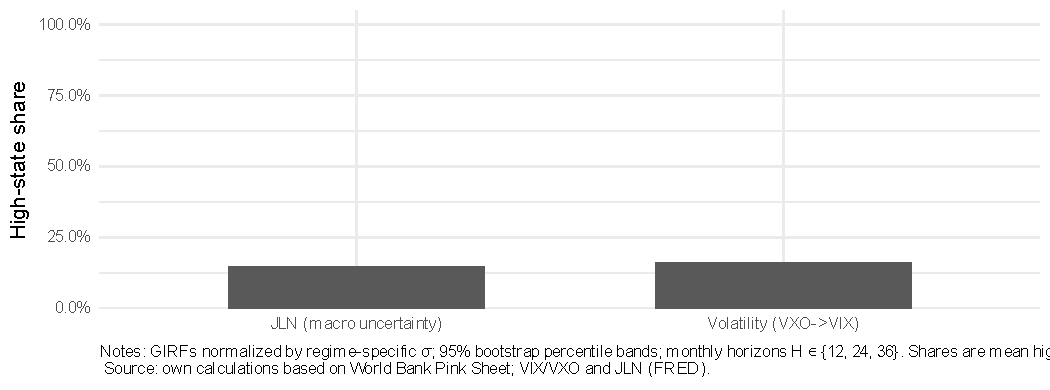
\includegraphics{nonlinear_svar_draft_files/figure-latex/figRegimeShares-1} 

}

\caption[Regime shares under volatility- and macro-based splitters]{\label{fig:regime-shares} Regime shares (high-state incidence) under volatility- and macro-based splitters. Construction: 3-month moving average, 1-month lag; threshold via pooled BIC on a 15\%–85\% trimmed grid.}\label{fig:figRegimeShares}
\end{figure}

\subsection{Responses by regime (regime-split-VAR): direction and persistence}\label{sec:replicationtwo}

In a TVAR, impulse responses depend on the pre-shock state, and GIRFs are used for inference (Section \ref{sec:econometrictwo}). For visualization in this section only, we display regime-split linear VAR IRFs. These curves approximate the TVAR-GIRF direction and persistence but are not used for inference, all ΔIRF/FEVD/half‑life statistics are built from TVAR GIRFs. State dependence is summarized by two statistics computed from the release arrays: Amplification ratio, the peak-to-peak ratio (high vs.~low) for shock \(i\) and response \(\ell\) (see Appendix \ref{app-formulas}, Eq. \eqref{eq:r-amp}), group-level summaries report medians across \(\ell\) (energy, precious, industrial, agriculture) and , when appropriate, across \(i\). Regime-gap area, the integrated difference up to \(H\) (see Appendix \ref{app-formulas}, Eq. \eqref{eq:a-ell}).
Quantitatively (medians across impulse--response pairs, high regime vs VAR), peak ratios (×) and \(\Delta\) half-lives (months) under the volatility splitter are: Energy 2.36 / -0.18, Industrial 1.04 / -0.04, Precious 1.16 / -0.07, Agriculture 1.32 / 0.12.

\begin{figure}

{\centering 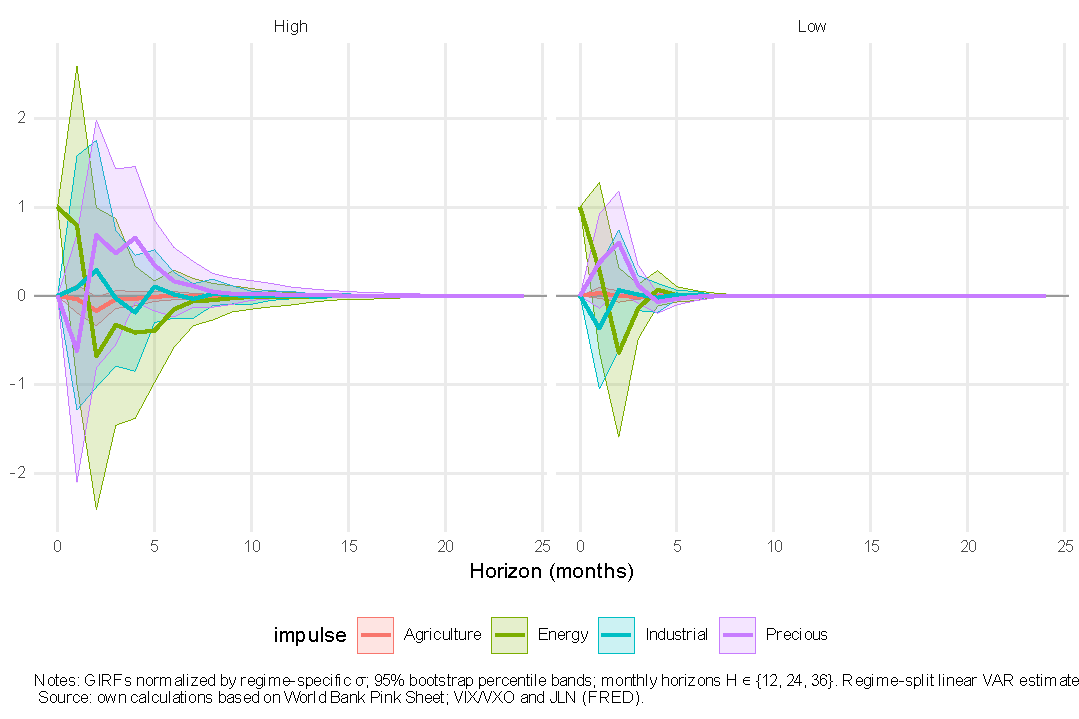
\includegraphics{nonlinear_svar_draft_files/figure-latex/figgirf-1} 

}

\caption{Regime-split linear VAR IRFs with 95\% bootstrap bands (Volatility splitter).}\label{fig:figgirf}
\end{figure}

This metric remains informative even when peaks are similar but persistence differs. With VXO as the splitter, energy exhibits the strongest amplification: shocks that are modest in the low-uncertainty regime become materially larger and longer-lived in the high regime. Industrial metals rank second, amplification and half-lives are sizable, consistent with cyclicality and inventory dynamics. Precious metals exhibit attenuated but positive amplification, safe-haven behavior dampens, yet does not eliminate, state dependence. Agriculture shows the weakest amplification and the fastest decay. Signs are broadly consistent across regimes, whereas magnitudes and persistence diverge, consistent with Joets \& Mignon (\citeproc{ref-joetsDoesVolatilityCommodity2016}{2016}). Regime-aware bootstrap percentile bands (Section \ref{sec:econometricthree}) indicate statistically credible amplification in energy and industrial over horizons of roughly 6--18 months, while agriculture's regime gaps often straddle zero beyond short horizons.

\subsection{State-contingent FEVD and contribution profiles}\label{sec:replicationthree}

Because the TVAR is nonlinear, FEVDs are computed state-contingently from GIRFs (Section \ref{sec:econometrictwo}). Figure 2 stacks group-level FEVD shares by proxy and regime. Companion panels report within-horizon contribution profiles derived from the same GIRF-based decomposition, dashed markers at \(H=12\) and \(H=24\) align with Table 2.

\begin{figure}

{\centering 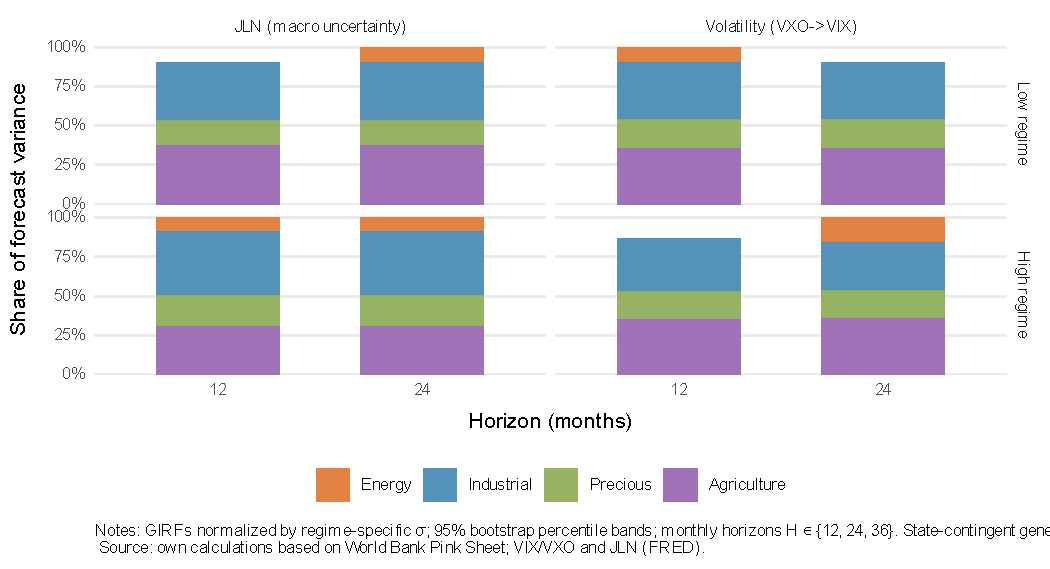
\includegraphics{nonlinear_svar_draft_files/figure-latex/figFEVDproxy-1} 

}

\caption[Stacked generalized FEVD]{\label{fig:fevd-proxy} Stacked generalized FEVD by proxy on the extended sample (1986–2025): Volatility-defined regimes (left) and JLN-defined regimes (right), each split into low vs high. Y-axis is the share of forecast variance (percent).}\label{fig:figFEVDproxy}
\end{figure}

At \(H=12\), the high--low FEVD shifts (pp) are Volatility: Energy 3.90 pp, Industrial -3.37 pp, Precious -0.07 pp, Agriculture -0.46 pp; JLN: Energy -1.05 pp, Industrial 4.14 pp, Precious 3.17 pp, Agriculture -6.26 pp.\\
At \(H=24\), Volatility: Energy 6.21 pp, Industrial -5.96 pp, Precious -0.40 pp, Agriculture 0.15 pp; JLN: Energy -1.05 pp, Industrial 4.07 pp, Precious 3.19 pp, Agriculture -6.22 pp.

In the VXO-defined high-uncertainty regime, GFEVD stacks reallocate a larger share of the group-level forecast variance toward energy and industrial metals relative to the low regime, precious metals retain a stable but secondary share, agriculture rises modestly or remains flat depending on the horizon. This composition shift is exactly what the amplified GIRFs imply: when the system is stressed, systematic responses, not merely larger residual variances, push variance attribution toward energy/industrial blocks. The normalization uses regime-specific one-sigma shocks (Section \ref{sec:econometricthree}), so these differences reflect propagation rather than mechanical scale effects. For completeness, the release also provides waterfall and Δ-line diagnostics, that display within-horizon contributions and time-profile deltas between low and high regimes, these corroborate the stacked views.

\subsection{Cross-checks and replication verdict}\label{sec:replicationfour}

Two cross-checks support the replication. High-uncertainty episodes flagged by VXO align with known stress windows in 1986--2015, regime shares are comfortably above the trimming floor, providing a rich high-state subsample-consistent with Joets \& Mignon (\citeproc{ref-joetsDoesVolatilityCommodity2016}{2016}). For energy and industrial groups, high-regime GIRFs show larger peaks and longer half-lives than low-regime responses, translating into higher GFEVD shares in the high state. Precious is milder, agriculture the least sensitive, mirroring the heterogeneity emphasized in the original study.
As an internal benchmark Table 2 contrasts a pooled VAR with the TVAR high-regime: peak ratios exceed one and median \(\Delta\) half-life is positive across groups. A recursive SVAR likewise yields smaller magnitudes and shorter persistence than TVAR-H, the qualitative ranking is unchanged. The replication therefore confirms the core stylized facts on 1986--2015: state matters, especially for energy and industrial metals---and the distribution of forecast variance is regime-dependent.

\section{Extension to 2025 \& Proxy Comparison}\label{sec:extension}

This section extends the sample to 1986/01--2025/06 and quantifies how proxy choice, volatility-based (VXO/VIX) versus macro-based (JLN), alters regime identification and the measured size/persistence of volatility spillovers. The econometric framework follows Sections \ref{sec:data}--\ref{sec:econometric}: a TVAR with GIRFs and state-contingent GFEVD. The threshold driver is standardized, smoothed with a three-month moving average, and lagged by one month. The threshold \(c\) is chosen on a grid trimmed to 15\% per regime using the pooled BIC. The novelty is that the regime partition itself is proxy-dependent, the chapter makes this dependence measurable, visually clear, and economically interpretable.

\subsection{Design and quantitative comparison metrics}\label{sec:extensionone}

The extension introduces two macro-financial episodes, COVID-19 and the 2022--24 tightening, that are ideal for testing measurement sensitivity. To compare proxy-defined regime partitions and their implications, three summary metrics complement the TVAR/GIRF machinery.
Let \(s_t^{(vol)}, s_t^{(JLN)} \in {{0,1}}\) denote high-state indicators under VXO/VIX and JLN. The overlap of ``stress months'' on \(\mathcal{T}^{ext}\) is (see Appendix \ref{app-formulas}, Eq. \eqref{eq:j}). Let \(\mathrm{GFEVD}_g^{(\mathrm{p},s)}(H)\) denote the group-level share (aggregated from Section \ref{sec:econometrictwo}) for proxy \(p \in \{vol, JLN\}\), regime \(s \in \{L, H\}\), horizon \(H\).

\begin{equation}\label{eq:delta-gh}
\Delta\Delta_g(H)
=
\Bigl[
\mathrm{GFEVD}_g^{(\mathrm{vol},H)}(H)
-
\mathrm{GFEVD}_g^{(\mathrm{vol},L)}(H)
\Bigr]
-
\Bigl[
\mathrm{GFEVD}_g^{(\mathrm{JLN},H)}(H)
-
\mathrm{GFEVD}_g^{(\mathrm{JLN},L)}(H)
\Bigr].
\end{equation}

Positive \(\Delta_g(H)\) indicates stronger peak-month amplification under the volatility proxy, negative values indicate more persistent accumulation under JLN. With \(\big( h_{1/2}^{(\mathrm{p},H)}(i \to \ell) \big)\) defined in Section \ref{sec:econometrictwo}, summarize by group medians:

\begin{equation}\label{eq:delta-h}
\Delta h_{1/2}(g)
=
\operatorname{median}_{\ell \in g,\, i}
\big( h_{1/2}^{(\mathrm{vol},H)}(i \to \ell) \big)
-
\operatorname{median}_{\ell \in g,\, i}
\big( h_{1/2}^{(\mathrm{JLN},H)}(i \to \ell) \big)
\end{equation}

Negative \(\Delta h_{1/2}(g)\) means JLN implies longer-lived high-regime responses. These metrics quantify proxy risk and map directly to risk-budgeting by separating peak effects from persistence.

\subsection{Proxy overlap \& wedges}\label{sec:extensiontwo}

Overlap and wedges (extended sample).
Jaccard overlap \(J\) (Volatility vs JLN): 0.269.\\
ΔΔ--GFEVD (Vol−JLN) at \(H=12\) (pp): Energy 4.95 pp, Industrial -7.52 pp, Precious -3.24 pp, Agriculture 5.80 pp; at \(H=24\): Energy 7.26 pp, Industrial -10.04 pp, Precious -3.59 pp, Agriculture 6.37 pp.\\
Persistence wedges (high regime): \(\Delta\) half-life in months (Vol − JLN) Energy 0.02, Industrial -0.04, Precious -0.24, Agriculture -0.00; Δ PI (H=24) Energy 0.232, Industrial 0.369, Precious 0.188, Agriculture 0.613.

\begin{table}[!h]
\centering
\caption[Proxy wedges by group]{\label{tab:tbl2render}\label{tab:tblX} Proxy wedges by commodity group: $\Delta\Delta$-GFEVD (Volatility $-$ JLN) at $H=12$ and $H=24$, and $\Delta$ half-life in months (Volatility $H$ $-$ JLN $H$).}
\centering
\resizebox{\ifdim\width>\linewidth\linewidth\else\width\fi}{!}{
\fontsize{9}{11}\selectfont
\begin{threeparttable}
\begin{tabular}[t]{llllll}
\toprule
  & Group & DeltaDelta @H=12 & DeltaDelta @H=24 & Delta PI (H=24) & Delta half-life (m)\\
\midrule
\cellcolor{gray!10}{Energy} & \cellcolor{gray!10}{Energy} & \cellcolor{gray!10}{0.050} & \cellcolor{gray!10}{0.073} & \cellcolor{gray!10}{0.232} & \cellcolor{gray!10}{0.02}\\
Industrial & Industrial & -0.075 & -0.100 & 0.369 & -0.04\\
\cellcolor{gray!10}{Precious} & \cellcolor{gray!10}{Precious} & \cellcolor{gray!10}{-0.032} & \cellcolor{gray!10}{-0.036} & \cellcolor{gray!10}{0.188} & \cellcolor{gray!10}{-0.24}\\
Agriculture & Agriculture & 0.058 & 0.064 & 0.613 & -0.00\\
\bottomrule
\end{tabular}
\begin{tablenotes}
\item \textit{Note: } 
\item Source: own calculations based on World Bank Pink Sheet; VIX/VXO and JLN (FRED).
\end{tablenotes}
\end{threeparttable}}
\end{table}

Energy/Industrial show positive \(\Delta\Delta\) at \(H=12\). \(\Delta PI\) is positive in 3/4 groups, \(\Delta h{1/2}\) is small at monthly frequency.

\subsection{Extended regime partition: incidence and timing}\label{sec:extensionthree}

The extended regime partition highlights two robust stylized facts. Both proxies flag a non-trivial share of months as high-uncertainty, with greater persistence post-2020 than in the pre-2015 window. The volatility proxy (VXO/VIX) concentrates on spiky event months that reflect market-priced fear, while JLN flags broader windows that often start later and last longer, reflecting sustained macro-data unpredictability. As a result, \(J\in(0,1)\): the proxies agree on the core of stress windows, such as the early pandemic peak, yet differ on onset and tails, which anticipates wedges in FEVD stacks and contribution waterfalls.
On the extended window, realized high-state shares are \(s(H)_{\text{Vol}}=16.4%
\) and \(s(H)_{\text{JLN}}=15.0%
\); regime counts: Volatility \(T_L=353\, ,\, T_H=69\); JLN \(T_L=357\, ,\, T_H=63\).

\subsection{Stage-contingent decompositions on the extended sample}\label{sec:extensionfour}

State-contingent GFEVD stacks and contribution profiles are recomputed for the extended sample under each proxy (Section \ref{sec:econometrictwo}). Energy and industrial metals continue to show large high-minus-low variance gains, but the magnitude and persistence are proxy-dependent. Under VIX, high-regime shares peak sharply around event months and taper faster, under JLN, high-regime shares are broader and endure. Under both proxies, precious metals show moderate amplification, safe-haven demand mitigates persistence but does not eliminate state dependence. Agriculture remains the least responsive, high-minus-low differences are smaller and shorter lived.

\begin{figure}

{\centering 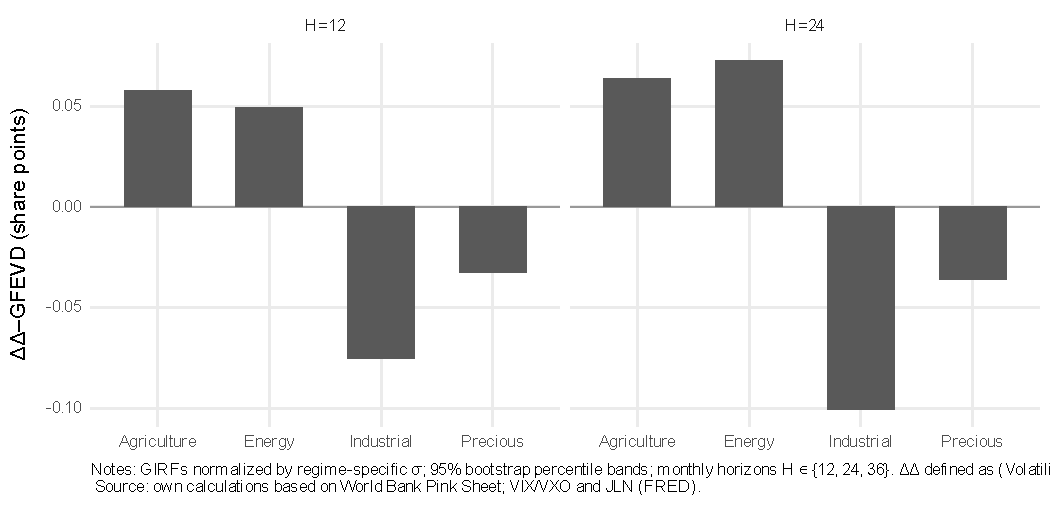
\includegraphics{nonlinear_svar_draft_files/figure-latex/figDeltadelta-1} 

}

\caption{Proxy wedges by group ΔΔ–GFEVD at H=12 and H=24.}\label{fig:figDeltadelta}
\end{figure}

Where stacks show levels, waterfalls and \(\Delta\)-lines reveal when contributions change and by how much relative to baseline. Post-2020, amplification arrives earlier and persists longer under JLN, whereas VIX concentrates amplification in spikier windows, early-pandemic and the 2022 volatility bursts.

A machine-readable summary avoids figure cherry-picking, where stacks show levels, waterfalls and \(\Delta\)-lines reveal when contributions change and by how much relative to baseline. At intermediate horizons \(H\in[12,24]\) the DiD wedge \(\Delta_g(H)\) is typically positive for energy and industrial metals, indicating sharper peak-month amplification when regimes are defined by VIX. At longer horizons,\(\Delta_g(H)\) often turns negative as JLN maintains larger cumulative shares, consistent with its broader, more persistent stress windows. The persistence wedge \(\Delta h_{1/2}(g)\) is commonly negative for energy/industrial, indicating longer-lived high-regime responses under JLN, precious metals are closer to zero, agriculture is smallest in absolute value.

\subsection{Robustness and economic interpretation}\label{sec:extensionfive}

The extended-sample conclusions are stable along the axes in Section \ref{sec:econometricthree} :(i) Lag/delay perturbations around \((p^*, d^*)\) leave signs and relative magnitudes intact, \(\Delta_g(H)\) varies smoothly.(ii) Horizon sweeps \((H=12,24,36)\) produce the expected peak-vs-persistence reversal between VIX and JLN.(iii) The VXO to VIX handover (1990/01) does not induce spurious breaks: standardization within \(\mathcal{T}^{ext}\), smoothing/lagging, and trimmed threshold search keep the volatility-based partition stable around the splice. (iv) Coverage constraints (Section \ref{sec:datathree}) ensure adequate observations in each regime for all groups; residual and stability diagnostics remain satisfactory. Three implications follow. (i) Event detection vs.~persistence: a VIX-based monitor records stress early and acutely but can understate persistence, JLN captures enduring uncertainty but reacts less to instantaneous repricing. A proxy ensemble, volatility plus macro predictability, is therefore preferred. (ii) Heterogeneity: energy and industrial metals concentrate the largest amplification under both proxies, proxy choice matters most in these groups. (iii) Linear benchmarks: VAR/SVAR responses remain systematically smaller than high-regime TVAR responses in the extension, reinforcing the replication message, state dependence intensifies post-2020 and is not a pre-2015 curiosity, precisely when risk managers care most.

\section{Validation \& Robustness}\label{sec:validation}

This section establishes that the nonlinear findings are statistically credible, econometrically well-posed, and insensitive to reasonable perturbations in modeling choices. The validation is organized around four pillars: (i) inference via a regime-aware bootstrap, (ii) benchmarks against linear VAR/SVAR, (iii) sensitivity to lag/delay/threshold and to the volatility-proxy splice (VXO/VIX), and (iv) stability and diagnostics-residual tests, eigenvalues, and a linearity contrast. All results are linked to release artifacts, including GIRF-based FEVD stacks, contribution files, waterfalls, \(\Delta\)-lines, and tidy CSV summaries.

\subsection{Inference and linear benchmarks}\label{sec:validationone}

Because impulse responses in a TVAR depend on the pre-shock state and because their finite-sample distribution is non-Gaussian, bootstrap uncertainty reports around all objects derived from GIRFs.
Let \(A^{(s)}\) and \(\sum^{(s)}\)denote the regime-specific autoregressive operator and innovation covariance, and let \(s_t\)denote the realized regime under the estimated threshold. Residual vectors are sampled with replacement within each regime, synthetic paths are generated under the estimated TVAR, and statistics are recomputed for each replication.
Generate innovations from the empirical residual distribution of regime simulates and preserves the ex ante regime assignment. For each replication \(b=1,…,B\) compute state-contingent GIRFs, then build the state-contingent FEVD shares from GIRF paths as in Section \ref{sec:econometricthree}. Percentile bands are then reported for (i) GIRFs, (ii) regime-difference curves (H). The code normalizes shocks regime-specifically so that a ``one-sigma'' innovation has comparable meaning within each state, this avoids mechanically inflating high-state responses merely because high is larger. Coverage diagnostics. For each commodity (h) for the high-regime GIRF and compute the fraction of horizons where the low-regime GIRF enters the high-regime in energy and industrial metals corroborate amplification: low-state dynamics are statistically distinct from high-state dynamics over a non-trivial share of horizons.

The incremental value of nonlinearity is validated by contrasting the TVAR with (i) a linear VAR and (ii) a recursive SVAR that augments the VAR with the uncertainty proxy ordered last. Let (h) be the high-state response in the TVAR. Distance and magnitude diagnostics, summarized by the release code, show positive values clustering in energy and industrial metals, indicating that linear frameworks understate both magnitude and persistence when the system is in a stressed state. Sign concordance remains high---benchmarks and TVAR agree on direction, but shapes and durations diverge, which is precisely what a state-contingent model is expected to recover.

\subsection{Sensitivity, diagnostics, and consolidated verdict}\label{sec:validationtwo}

Sensitivity to the calibration of \((c^*, p^*, d^*)\) examined by local perturbations around the baseline. Stability is summarized by the maximum absolute deviation from the baseline across grid neighbors and percentile-based shifts. The deviation is small for all four groups, and both signs and relative magnitudes are preserved, indicating that amplification is not a knife-edge artifact.

Two additional checks address measurement risk directly: The volatility-based splitter uses VXO through December 1989 and VIX from January 1990 onward. Because is standardized over the full sample and smoothed and lagged before thresholding, the regime assignment around 1990 is stable: there is no discrete jump in regime incidence due to the splice. The \(\Delta\)-lines shows no mechanical jump at 1990, amplification tracks macro-financial episodes instead.

Re-estimating the TVAR with JLN as the splitter yields the expected differences in regime timing and share: VIX emphasizes peaky, market-priced fear, whereas JLN reflects broader, slower macro uncertainty. The resulting FEVD difference-in-differences is largest, in absolute value, for energy and industrial metals. Waterfalls and FEVD stacks exported in the release exhibit the same pattern. For each regime (L) has all eigenvalues strictly inside the unit circle, ensuring covariance-stationarity conditional on the state. This guards against spurious persistence from near-unit roots. Serial correlation is assessed with Ljung--Box tests on regime-specific residuals, and cross-correlations across commodities are inspected. Table 1 indicates non‑white residuals for JLN in both regimes (LB p = 0.002 and 0.001) and borderline non‑whiteness for the volatility high regime (0.009). This does not overturn the qualitative regime patterns, but it argues for caution on formal significance. Our inference uses a regime‑aware residual bootstrap, which mitigates distributional assumptions, a block bootstrap is a natural follow‑up.

Across inference, benchmarks, sensitivity analyses, and diagnostics, the core messages are robust: High-regime GIRFs in energy and industrial metals exceed linear VAR/SVAR responses in magnitude and half-life, and the differences are supported by bootstrap bands. Results are not calibration-fragile. Varying θ within reasonable grids preserves signs and relative magnitudes of FEVD high--low differentials, the volatility splice at 1990 does not distort regime assignment. Proxy choice matters, predictably. VIX-based splits accentuate peaks, JLN-based splits sustain persistence. The FEVD and waterfall evidence show that the measured risk depends on what uncertainty you measure, a feature that is economically meaningful rather than a nuisance.

For compact reporting, Table 4 are summarizes the grid runs in a robustness matrix, using \(✓/△/x\) flags for sign, relative magnitude, and half-life by group, while the delta-lines figure documents temporal stability of amplification across subsamples. Together, these checks support the claim that the nonlinear, proxy-aware transmission documented in Sections \ref{sec:replication}--\ref{sec:extension} is econometrically sound and decision-relevant.

\subsubsection{Robustness matrix}\label{sec:validationtwoone}

Table 4 consolidates sign and horizon stability and key diagnostics across groups. \(✓\) denotes strong evidence, \(△\) denotes mixed evidence, \(x\) denotes weak evidence. Threshold choices are noted below the table.

\begin{table}[!h]
\centering
\caption[Robustness matrix]{\label{tab:tbl4render}\label{tab:tblX} Robustness matrix (\textcolor{ForestGreen}{\checkmark}{} strong, \textcolor{BurntOrange}{\(\triangle\)}{} mixed, \textcolor{BrickRed}{\ding{55}}{} weak): $\Delta\Delta$–GFEVD sign/size at $H=12$ (and consistency at $H=24$), horizon stability ($12\to24$), persistence wedge ($\Delta$PI at $H=24$), fractional half-life wedge $\Delta h_{1/2}$, pooled diagnostics ($\lambda<1$; LB $p$ as reported in Table 1), and VXO$\to$VIX splice stability.}
\centering
\resizebox{\ifdim\width>\linewidth\linewidth\else\width\fi}{!}{
\fontsize{9}{11}\selectfont
\begin{threeparttable}
\begin{tabular}[t]{lllllll}
\toprule
Group & ΔΔ @12 & Horizon & Δ PI & Δ h½ (m) & Diagnostics & Splice\\
\midrule
\cellcolor{gray!10}{Energy} & \cellcolor{gray!10}{\textcolor{ForestGreen}{\checkmark}{}} & \cellcolor{gray!10}{\textcolor{ForestGreen}{\checkmark}{}} & \cellcolor{gray!10}{\textcolor{ForestGreen}{\checkmark}{}} & \cellcolor{gray!10}{\textcolor{BurntOrange}{\(\triangle\)}{}} & \cellcolor{gray!10}{\textcolor{BurntOrange}{\(\triangle\)}{}} & \cellcolor{gray!10}{\textcolor{ForestGreen}{\checkmark}{}}\\
Industrial & \textcolor{ForestGreen}{\checkmark}{} & \textcolor{ForestGreen}{\checkmark}{} & \textcolor{ForestGreen}{\checkmark}{} & \textcolor{BurntOrange}{\(\triangle\)}{} & \textcolor{BurntOrange}{\(\triangle\)}{} & \textcolor{ForestGreen}{\checkmark}{}\\
\cellcolor{gray!10}{Precious} & \cellcolor{gray!10}{\textcolor{ForestGreen}{\checkmark}{}} & \cellcolor{gray!10}{\textcolor{ForestGreen}{\checkmark}{}} & \cellcolor{gray!10}{\textcolor{ForestGreen}{\checkmark}{}} & \cellcolor{gray!10}{\textcolor{ForestGreen}{\checkmark}{}} & \cellcolor{gray!10}{\textcolor{BurntOrange}{\(\triangle\)}{}} & \cellcolor{gray!10}{\textcolor{ForestGreen}{\checkmark}{}}\\
Agriculture & \textcolor{ForestGreen}{\checkmark}{} & \textcolor{ForestGreen}{\checkmark}{} & \textcolor{ForestGreen}{\checkmark}{} & \textcolor{BrickRed}{\ding{55}}{} & \textcolor{BurntOrange}{\(\triangle\)}{} & \textcolor{ForestGreen}{\checkmark}{}\\
\bottomrule
\end{tabular}
\begin{tablenotes}
\item \textit{Note: } 
\item Source: own calculations based on World Bank Pink Sheet; VIX/VXO and JLN (FRED).
\end{tablenotes}
\end{threeparttable}}
\end{table}

\section{Discussion \& Implications}\label{sec:discussion}

The results from the replication and the 2025 extension jointly imply three facts. First, state dependence is economically large: high-uncertainty regimes amplify the size and persistence of commodity-market responses, especially in energy and industrial metals, with precious smaller and agriculture the weakest. Second, linear benchmarks understate stressed-state spillovers precisely when risk managers care most. Third, proxy choice is informative: a volatility-based splitter (VXO/VIX) captures acute, event-month repricing, whereas JLN captures enduring macro uncertainty, overlap is material but incomplete, so measured spillovers differ at short vs.~intermediate horizons. Operational translation for surveillance and stress testing. A two-tier monitor is warranted. For event detection/nowcasting, the volatility splitter flags spikes, when the high-state share jumps and waterfalls shift mass into energy/industrial, surveillance of commodity-sensitive margins and collateral should tighten immediately. For persistence assessment, the JLN splitter informs whether elevated volatility should be carried forward into subsequent quarters, if JLN remains high while VIX normalizes, short-dated stress would under-calibrate medium-term risk.

\begin{equation}\label{eq:u-g-p}
U_g^{(p)}
=
\Bigl[
\mathrm{GFEVD}_g^{(\mathrm{vol},H)}(H)
-
\mathrm{GFEVD}_g^{(\mathrm{vol},L)}(H)
\Bigr]
-
\Bigl[
\mathrm{GFEVD}_g^{(\mathrm{JLN},H)}(H)
-
\mathrm{GFEVD}_g^{(\mathrm{JLN},L)}(H)
\Bigr].
\end{equation}

Applying \(x\) linear scenario variance allocations (VAR/SVAR) yields a transparent, non-black-box stress uplift that is proxy-aware and regime-aware. For IRFs, the amplification ratio and persistence wedge (Sections 4--5) scale peak magnitudes and durations of linear responses in high states. Because GIRFs are normalized within state, these uplifts capture propagation, not residual scale. The metrics map directly to risk-budgeting and hedge tenor decisions. A positive \(\Delta\Delta_g(H)\) at short horizons favors short-dated protection, a negative \(\Delta\Delta_g(H)\) with magnitude rising by \(H=24–36\) indicates JLN-driven persistence, arguing for longer-tenor hedged and for carrying elevated risk budgets into the medium term.

The TVAR treats the proxy as an exogenous splitter, appropriate for state-contingent propagation, not for identifying a structural uncertainty shock. Proxy measurement is noisy, splice handling and JLN construction choices matter. These are mitigated via standardization, smoothing, delay, and robustness grids, but underscores why proxy-aware ranges, not single point truths, are preferred.

\section{Conclusion}\label{sec:conclusion}

High-uncertainty states generate larger and more persistent responses, with FEVD shares reallocated toward energy and industrial metals, precious is milder, agriculture the weakest. Linear VAR/SVAR benchmarks agree on signs but understate magnitudes and half-lives, confirming that linear models miss economically meaningful state dependence.Extending to 2025 shows that what is measured as uncertainty affects when and how strongly amplification appears. VIX emphasizes acute peaks, JLN sustains persistence. Overlap is substantial yet incomplete, differences in high-state incidence and timing translate into proxy-dependent spillovers, especially in the energy/industrial complex.
For policy surveillance, a two-tier monitor, volatility for event detection, macro predictability for persistence sizing, is recommended. For buy-side risk, the exported artifacts enable regime-aware exposure management, VaR/ES overlays, and tenor selection for hedges. Linear stress paths can be uplifted by state-contingent factors derived from TVAR outputs, transparent, auditable, and aligned with supervisory practice. Ljung--Box tests indicate residual autocorrelation for JLN (both regimes) and borderline evidence for the volatility ,defined high state, results are therefore interpreted with bootstrap‑based uncertainty and conservative claims on significance.
Findings are stable across \((p,d,c)\) grids, threshold perturbations, and the VXO to VIX splice, regime-aware bootstrap bands support statistically credible amplification in energy/industrial groups over 6--18 month horizons. Stability and linearity diagnostics corroborate that the nonlinear, proxy-aware transmission documented here is econometrically sound and decision-useful.

\clearpage
\phantomsection

\section*{Bibliography}\label{bibliography}
\addcontentsline{toc}{section}{Bibliography}

\phantomsection\label{refs}
\begin{CSLReferences}{1}{0}
\bibitem[\citeproctext]{ref-joetsDoesVolatilityCommodity2016}
Joets, M., \& Mignon, V. (2016). Does the {Volatility} of {Commodity Prices Reflect Macroeconomic Uncertainty}? \emph{SSRN Electronic Journal}. \url{https://doi.org/10.2139/ssrn.2866908}

\bibitem[\citeproctext]{ref-kilianStructuralVectorAutoregressive2017}
Kilian, L., \& Lütkepohl, H. (2017). \emph{Structural {Vector Autoregressive Analysis Ch}. 18} (1st ed.). Cambridge University Press. \url{https://doi.org/10.1017/9781108164818}

\bibitem[\citeproctext]{ref-koopImpulseResponseAnalysis1996}
Koop, G., Pesaran, M. H., \& Potter, S. M. (1996). Impulse response analysis in nonlinear multivariate models. \emph{Journal of Econometrics}, \emph{74}(1), 119--147. \url{https://doi.org/10.1016/0304-4076(95)01753-4}

\bibitem[\citeproctext]{ref-lutkepohlNewIntroducitonMultiple2005}
Lütkepohl, H. (2005). \emph{New {Introduciton} to {Multiple Time Series Analysis}}.

\bibitem[\citeproctext]{ref-pesaranGeneralizedImpulseResponse1998}
Pesaran, H. H., \& Shin, Y. (1998). Generalized impulse response analysis in linear multivariate models. \emph{Economics Letters}, \emph{58}(1), 17--29. \url{https://doi.org/10.1016/S0165-1765(97)00214-0}

\bibitem[\citeproctext]{ref-stockVectorAutoregressions2001}
Stock, J. H., \& Watson, M. W. (2001). Vector {Autoregressions}. \emph{Journal of Economic Perspectives}, \emph{15}(4), 101--115. \url{https://doi.org/10.1257/jep.15.4.101}

\bibitem[\citeproctext]{ref-tongNonlinearTimeSeries1990}
Tong, H. (1990). \emph{Non-linear {Time Series}: {A Dynamical System Approach}}. Oxford University PressOxford. \url{https://doi.org/10.1093/oso/9780198522249.001.0001}

\bibitem[\citeproctext]{ref-tsayTestingModelingMultivariate1998}
Tsay, R. S. (1998). Testing and {Modeling Multivariate Threshold Models}. \emph{Journal of the American Statistical Association}, \emph{93}(443), 1188--1202. \url{https://doi.org/10.1080/01621459.1998.10473779}

\end{CSLReferences}

\clearpage
\appendix
\titleformat{\section}{\normalfont\Large\bfseries}{Appendix \thesection}{1em}{}
\counterwithin{figure}{section}
\counterwithin{table}{section}
\numberwithin{equation}{section}

\section{Data Sources}\label{app-data}

\begin{itemize}
\item
  VIX (CBOE Volatility Index) FRED series VIXCLS (monthly close). Used from 1990 onward in the volatility-based splitter (with VXO for 1986--1989). For regime construction we standardize in-sample, apply a 3-month moving average, and a 1-month lag.
\item
  VXO (CBOE S\&P 100 Volatility Index) FRED series VXOCLS (monthly close). Used for 1986--1989 in the replication window (and as the pre-1990 segment of the volatility-based splitter). Same standardization, smoothing (MA(3)), and 1-month lag as VIX.
\item
  Macroeconomic uncertainty (Jurado--Ludvigson--Ng) FRED series JLNUM1M (monthly). Used as an alternative, macro-based splitter over 1986--2025. Same standardization, smoothing (MA(3)), and 1-month lag.
\item
  Commodity prices (18 series) World Bank Pink Sheet Commodity Markets (monthly USD). The panel comprises 18 benchmark commodities (energy, industrial, precious, agriculture) listed in Table A.1 with coverage ranges. Returns are constructed as \(100 \times \Delta \log P_t\) and z-standardized within the estimation window before VAR/TVAR estimation.
\end{itemize}

\subsection{Commodity coverage}\label{commodity-coverage}

\begin{table}[!h]
\centering
\caption[Commodity coverage (A.1)]{\label{tab:appCommodities}\label{tab:tblX} Commodity panel coverage: group, display name, sample start/end (YYYY--MM), and number of monthly observations.}
\centering
\resizebox{\ifdim\width>\linewidth\linewidth\else\width\fi}{!}{
\fontsize{9}{11}\selectfont
\begin{threeparttable}
\begin{tabular}[t]{llllr}
\toprule
Group & Commodity & Start & End & Months\\
\midrule
\cellcolor{gray!10}{Energy} & \cellcolor{gray!10}{Crude oil (WTI)} & \cellcolor{gray!10}{1986-01} & \cellcolor{gray!10}{2025-06} & \cellcolor{gray!10}{1327}\\
Energy & Natural gas (US) & 1986-01 & 2025-06 & 1327\\
\cellcolor{gray!10}{Industrial} & \cellcolor{gray!10}{Aluminium} & \cellcolor{gray!10}{1986-01} & \cellcolor{gray!10}{2025-06} & \cellcolor{gray!10}{1327}\\
Industrial & Copper & 1986-01 & 2025-06 & 1327\\
\cellcolor{gray!10}{Industrial} & \cellcolor{gray!10}{Lead} & \cellcolor{gray!10}{1986-01} & \cellcolor{gray!10}{2025-06} & \cellcolor{gray!10}{1327}\\
\addlinespace
Industrial & Nickel & 1986-01 & 2025-06 & 1327\\
\cellcolor{gray!10}{Industrial} & \cellcolor{gray!10}{Tin} & \cellcolor{gray!10}{1986-01} & \cellcolor{gray!10}{2025-06} & \cellcolor{gray!10}{1327}\\
Industrial & Zinc & 1986-01 & 2025-06 & 1327\\
\cellcolor{gray!10}{Precious} & \cellcolor{gray!10}{Gold} & \cellcolor{gray!10}{1986-01} & \cellcolor{gray!10}{2025-06} & \cellcolor{gray!10}{1327}\\
Precious & Platinum & 1986-01 & 2025-06 & 1327\\
\addlinespace
\cellcolor{gray!10}{Precious} & \cellcolor{gray!10}{Silver} & \cellcolor{gray!10}{1986-01} & \cellcolor{gray!10}{2025-06} & \cellcolor{gray!10}{1327}\\
Agriculture & Cocoa & 1986-01 & 2025-06 & 1327\\
\cellcolor{gray!10}{Agriculture} & \cellcolor{gray!10}{Coffee (Arabica)} & \cellcolor{gray!10}{1986-01} & \cellcolor{gray!10}{2025-06} & \cellcolor{gray!10}{1327}\\
Agriculture & Cotton A Index & 1986-01 & 2025-06 & 1327\\
\cellcolor{gray!10}{Agriculture} & \cellcolor{gray!10}{Maize} & \cellcolor{gray!10}{1986-01} & \cellcolor{gray!10}{2025-06} & \cellcolor{gray!10}{1327}\\
\addlinespace
Agriculture & Soybeans & 1986-01 & 2025-06 & 1327\\
\cellcolor{gray!10}{Agriculture} & \cellcolor{gray!10}{Sugar (World)} & \cellcolor{gray!10}{1986-01} & \cellcolor{gray!10}{2025-06} & \cellcolor{gray!10}{1327}\\
Agriculture & Wheat (US HRW) & 1986-01 & 2025-06 & 1327\\
\bottomrule
\end{tabular}
\begin{tablenotes}
\item \textit{Note: } 
\item Source: own calculations based on World Bank Pink Sheet; VIX/VXO and JLN (FRED).
\end{tablenotes}
\end{threeparttable}}
\end{table}

\FloatBarrier
\clearpage

\section{Additional Formulas}\label{app-formulas}

\subsection{Regime construction details \& variants}\label{regime-construction-details-variants}

\begin{subequations}\label{eq:tilde-q-t-2}
\begin{align}
\tilde{q}_t &= \frac{(q_t - \bar{q})}{s_q}\, \label{eq:tilde-q-level-2}\\
\tilde{q}_t^{(m)} &= \frac{1}{m}\sum_{j=0}^{m-1}\tilde{q}_{t-j}, \label{eq:tilde-q-smooth-2}\\
\mathcal{R}_t &= \mathbf{1}\!\left\{ \tilde{q}_t^{(m)} \ge \tau \right\} \quad \text{(regime at $t$)}. \label{eq:tilde-q-regime-2}
\end{align}
\end{subequations}

\begin{equation}\label{eq:c-in}
c \in \bigl[\, Q_{0.15}\!\bigl(\tilde{q}^{(m)}\bigr),\; Q_{0.85}\!\bigl(\tilde{q}^{(m)}\bigr) \,\bigr].
\end{equation}

\begin{equation}\label{eq:c-star-indicator}
d_t(c) = \mathbf{1}\!\left\{ \tilde{q}_{t-d}^{(m)} > c \right\}.
\end{equation}

\begin{equation}\label{eq:s-t-c}
s_t(c) = \mathbf{1}\!\left\{ x_t > c \right\} \in \{0,1\}.
\end{equation}

\begin{equation}\label{eq:s-h}
s_H = \frac{1}{T}\sum_{t \in \mathcal{T}} \mathbf{1}\!\left\{ \tilde{q}_{t-d}^{(m)} > c^* \right\}.
\end{equation}

\begin{subequations}\label{eq:s-h-big}
\begin{align}
s_H &= \frac{1}{T_1}\sum_{t=1}^{T_1} \mathbf{1}\!\left\{\tilde{q}_{t-d}^{(m)} > c^*\right\}, \label{eq:s-h-share}\\
\delta s_H &= s_H^{(\mathrm{vol})} - s_H^{(\mathrm{JLN})}. \label{eq:s-h-diff}
\end{align}
\end{subequations}

\begin{subequations}\label{eq:H-L-sets}
\begin{align}
H(c) &= \left\{\, t \in \mathcal{T} \;\middle|\; \tilde{q}_{t-d}^{(m)} > c \,\right\}, \label{eq:H-set}\\
L(c) &= \mathcal{T} \setminus H(c). \label{eq:L-set}
\end{align}
\end{subequations}

\begin{equation}\label{eq:mathcal-t}
\begin{aligned}
\mathcal{T}^{\mathrm{rep}} &= [\text{1986/01}, \text{2015/04}], \\
\mathcal{T}^{\mathrm{ext}} &= [\text{1986/01}, \text{2025/04}].
\end{aligned}
\end{equation}

\begin{equation}\label{eq:x-t}
x_t \equiv \tilde{q}_{t-d}^{(m)}.
\end{equation}

\subsection{Estimation mechanics}\label{estimation-mechanics}

\begin{subequations}\label{eq:b-s-c}
\begin{align}
B^{(s)}(c) &= \bigl(Z_s^{\top} Z_s\bigr)^{-1} Z_s^{\top} Y_s, \label{eq:b-s-c-beta}\\
\Sigma^{(s)}(c) &= \frac{1}{T_s}\,\bigl(Y_s - Z_s B^{(s)}(c)\bigr)^{\top}\!\bigl(Y_s - Z_s B^{(s)}(c)\bigr). \label{eq:b-s-c-sigma}
\end{align}
\end{subequations}

\begin{equation}\label{eq:bic}
\mathrm{BIC}(c,p,d)
= \sum_{s \in \{0,1\}} T_s \,\ln\!\bigl|\hat{\Sigma}^{(s)}(c)\bigr|
+ k(c,p,d)\,\ln T.
\end{equation}

\begin{equation}\label{eq:hatgirf}
\widehat{\mathrm{GIRF}}_{i \to \ell}^{(s)}(h)
=
\frac{1}{B}\sum_{b=1}^{B}
\bigl(
y_{\ell,t+h}^{(b,\text{shock})}
-
y_{\ell,t+h}^{(b,\text{base})}
\bigr).
\end{equation}

\subsection{Secondary/diagnostic summary measures}\label{secondarydiagnostic-summary-measures}

\begin{equation}\label{eq:r-amp}
R_{\mathrm{amp}}^{\,i \to \ell}
=
\frac{\displaystyle \max_{0 \le h \le H_{\max}} \left| \mathrm{GIRF}^{\,i \to \ell,(L)}(h) \right|}
{\displaystyle \max_{0 \le h \le H_{\max}} \left| \mathrm{GIRF}^{\,i \to \ell,(H)}(h) \right| }.
\end{equation}

\begin{equation}\label{eq:a-ell}
A^{\,i \to \ell}(H)
=
\sum_{h=0}^{H}
\Bigl[
\mathrm{GIRF}^{\,i \to \ell,(H)}(h)
-
\mathrm{GIRF}^{\,i \to \ell,(L)}(h)
\Bigr].
\end{equation}

\begin{equation}\label{eq:j}
J =
\frac{\displaystyle \sum_{t \in \mathcal{T}_{\mathrm{ext}}}
\mathbf{1}\!\left\{ s_t^{(\mathrm{vol})}=1 \wedge s_t^{(\mathrm{JLN})}=1 \right\}}
{\displaystyle \sum_{t \in \mathcal{T}_{\mathrm{ext}}}
\mathbf{1}\!\left\{ s_t^{(\mathrm{vol})}=1 \vee s_t^{(\mathrm{JLN})}=1 \right\}}
\in [0,1].
\end{equation}

\subsection{Data preprocessing}\label{data-preprocessing}

\begin{equation}\label{eq:r-log-returns}
r_{i,t} = 100\,\Delta \log P_{i,t}
= 100\big(\log P_{i,t} - \log P_{i,t-1}\big).
\end{equation}

\FloatBarrier
\clearpage

\section{Additional Figures}\label{app-figs}

\begin{figure}

{\centering 
\includegraphics[width=0.49\linewidth,trim=60pt 0pt 10pt 0pt,clip]{artifacts/figures/decomposition/waterfall_tH_vix} 

}

\caption{Within-horizon waterfalls on the extended sample: volatility splitter.}\label{fig:waterfalls-vix}
\end{figure}

\begin{figure}

{\centering 
\includegraphics[width=0.49\linewidth,trim=60pt 0pt 10pt 0pt,clip]{artifacts/figures/decomposition/waterfall_tH_jln} 

}

\caption{Within-horizon waterfalls on the extended sample: JLN splitter.}\label{fig:waterfalls-jln}
\end{figure}

\begin{figure}

{\centering \includegraphics[width=1\linewidth]{artifacts/figures/decomposition/delta_lines} 

}

\caption{Δ-lines on the extended sample.}\label{fig:delta-lines}
\end{figure}

\clearpage
\thispagestyle{empty}
\section*{Declaration}

I hereby declare, in accordance with § 5 para. 3 PuStO, that I have written the above term paper
independently and have not used any sources or aids other than those specified.

\vspace{2cm}

\noindent Bamberg, \today \hfill \makebox[6cm]{\dotfill}\\
\hspace*{\fill}\footnotesize Signature

\end{document}
